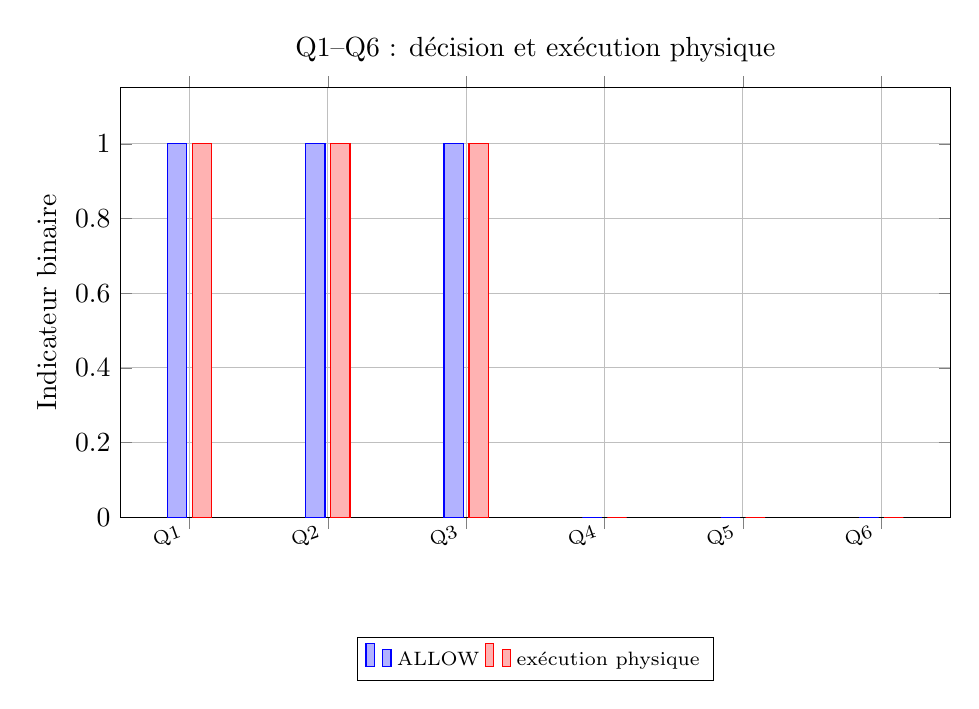
\begin{tikzpicture}
\begin{axis}[ybar,
bar width=7pt,
width=\linewidth,
height=0.58\linewidth,
title={Q1--Q6 : décision et exécution physique},
ylabel={Indicateur binaire},
xtick={0,1,2,3,4,5},
xticklabels={{Q1},{Q2},{Q3},{Q4},{Q5},{Q6}},
x tick label style={rotate=20,anchor=east,font=\scriptsize},
grid=major,
legend style={font=\scriptsize,at={(0.5,-0.28)},anchor=north,legend columns=2},
ymin=0,
ymax=1.15]
\addplot+ coordinates {(0,1) (1,1) (2,1) (3,0) (4,0) (5,0)};
\addlegendentry{ALLOW}
\addplot+ coordinates {(0,1) (1,1) (2,1) (3,0) (4,0) (5,0)};
\addlegendentry{exécution physique}
\end{axis}
\end{tikzpicture}
